% https://github.com/cohomolo-gy/cats-in-context/blob/master/chapter-2/Chapter%202%20Solutions.tex

\documentclass[11pt]{report}
\usepackage{classicthesis}

\usepackage{bbding} % for flower. 
\usepackage{physics}
\usepackage{amsmath,amssymb}
\usepackage{graphicx}
\usepackage{makeidx}
\usepackage{algpseudocode}
\usepackage{algorithm}
\usepackage{listing}
\usepackage{minted}
\usepackage{cancel}
\usepackage{quiver}
\usepackage{booktabs}   %% For formal tables:
                        %% http://ctan.org/pkg/booktabs
\usepackage{subcaption} %% For complex figures with subfigures/subcaptions
                        %% http://ctan.org/pkg/subcaption
\usepackage{enumitem}
%\usepackage{minted}
%\newminted{fortran}{fontsize=\footnotesize}

\usepackage{xargs}
\usepackage[colorinlistoftodos,prependcaption,textsize=tiny]{todonotes}

\usepackage{hyperref}
\hypersetup{
    colorlinks,
    citecolor=blue,
    filecolor=blue,
    linkcolor=blue,
    urlcolor=blue
}

\usepackage{epsfig}
\usepackage{tabularx}
\usepackage{latexsym}
\newcommand\ddfrac[2]{\frac{\displaystyle #1}{\displaystyle #2}}
\newcommand{\N}{\ensuremath{\mathbb{N}}}
\newcommand{\Z}{\ensuremath{\mathbb{Z}}}
\newcommand{\Q}{\ensuremath{\mathbb{Q}}}
\newcommand{\R}{\ensuremath{\mathbb R}}
\newcommand{\coT}{\ensuremath{T^*}}
\newcommand{\Lie}{\ensuremath{\mathfrak{L}}}
\newcommand{\Vectorfield}{\ensuremath{\mathfrak{X}}}
\newcommand{\pushforward}[1]{\ensuremath{{#1}_{\star}}}
\newcommand{\pullback}[1]{\ensuremath{{#1}^{\star}}}
\newcommand{\vectorfield}{\ensuremath{\mathfrak{X}}}

\newcommand{\pushfwd}[1]{\pushforward{#1}}
\newcommand{\pf}[1]{\pushfwd{#1}}

\newcommand{\boldX}{\ensuremath{\mathbf{X}}}
\newcommand{\boldY}{\ensuremath{\mathbf{Y}}}


\newcommand{\cat}[1]{\mathsf{#1}}
\newcommand{\functor}[3]{#1 : \cat{#2} \to \cat{#3}}
\newcommand{\functordef}{\functor{F}{C}{D}}
\newcommand{\cc}{\cat{C}}
\renewcommand{\dd}{\cat{D}}
\newcommand{\ee}{\cat{E}}
\newcommand{\ccat}{\cat{Cat}}
\newcommand{\cset}{\cat{Set}}
\newcommand{\subcat}[2]{\bm{ \mathsf{#1}}_{\bm{ \mathsf{#2}}}}
\renewcommand{\op}[1]{#1^{\text{op}}}
\newcommand{\inv}[1]{#1^{-1}}
\newcommand{\opc}{\op{\cc}}
\newcommand{\opd}{\op{\dd}}
\newcommand{\ope}{\op{\ee}}
\newcommand{\mono}{\rightarrowtail}
\newcommand{\epi}{\twoheadrightarrow}
\newcommand{\bg}{\cat{BG}}
\newcommand{\bgg}{\cat{BG'}}
\newcommand{\nt}{\Rightarrow}
%\newcommand{\ant}[2]{\alpha : F \nt G} 
%\newcommand{\bnt}[2]{\beta : F \nt G} 
%\newcommand{\anti}[2]{\alpha : F \cong G} 
%\newcommand{\bnti}[2]{\beta : F \cong G} 
\newcommand{\zero}{\mathbb{0}}
\newcommand{\one}{\mathbb{1}}
\newcommand{\two}{\mathbb{2}}
\newcommand{\three}{\mathbb{3}}



\newcommand{\G}{\ensuremath{\mathcal{G}}}
% \newcommand{\braket}[2]{\ensuremath{\left\langle #1 \vert #2 \right\rangle}}


\def\qed{$\Box$}
\newtheorem{theorem}{Theorem}
\newtheorem{corollary}[theorem]{Corollary}
\newtheorem{definition}[theorem]{Definition}
\newtheorem{lemma}[theorem]{Lemma}
\newtheorem{observation}[theorem]{Observation}
\newtheorem{remark}[theorem]{Remark}
\newtheorem{example}[theorem]{Example}
\newtheorem{exercise}[theorem]{Exercise}
 
% \newcommand{\proof}[1][]{\emph{Proof #1}\textbf{:} }
\newcommand*{\question}[1]{\leavevmode\newline \textbf{Question #1.}}
\newcommand*{\proof}[1]{\leavevmode\newline \textbf{Proof #1}}
\newcommand*{\answer}{\leavevmode\newline \textbf{Answer} }

\newcommand{\X}{\ensuremath{\mathfrak{X}}}
\newcommand{\comma}{\downarrow}

\title{Category theory in context}
\author{Siddharth Bhat}
\date{Monsoon, second year of the plague}


\begin{document}
\maketitle
\tableofcontents
\chapter{Categories, Functors, Natural transformations}
\section{Abstract and concrete categories}
\section{Duality}
\subsection{Musing}
How does one remember mono is is $gk = gl \implies k = l$ and vice versa?

\subsection{Solutions}
\question{Lemma 1.2.3} $f: x \to y$ is an isomorphism iff it defines a bijection $f_*: C(c, x) \to C(c, y)$.


\proof[($f$ is iso $\implies$ post composition with $f$ induces bijection)]
Let $f: x \to y$ be an isomorphism. Thus we have an inverse arrow $g: y \to x$ such that $fg = id_y$, $gf = id_x$.
The map: $$C(c, x) \xrightarrow{f*} C(c, y): (\alpha: c \to x) \mapsto (f\alpha: c \to y)$$
has a two sided inverse:

$$
C(c, y) \xrightarrow{g*} C(c, x): (\beta: c \to y) \mapsto (g\beta: c \to x)
$$

which can be checked as $g_*(f_*(\alpha)) = g_*(f\alpha) = gf\alpha = id_x\alpha = \alpha$, and similarly for $f_*(g_*(\beta))$.
Hence we are done, as the iso induces a bijection of hom-sets.
\qed


\proof[(post-composition with $f$ is bijection implies $f$ is iso)]
We are given that the post composition by $f$, $f_*: C(c, x) \rightarrow C(c, y)$ is a bijection.
We need to show that $f$ is an isomorphism, which means that there exists a function $g$ such that $fg = id_y$ and $gf = id_x$.
Since post-composition is a bijection for all $c$, pick $c = y$. This tells us that the post-composition 
$f_*: C(y, x) \rightarrow C(y, y)$ is a bijection. Since $id_y \in C(y, y)$, $id_y$ an inverse image $g \equiv f_*^{-1}(id_y)$. 
[We choose to call this map $g$]. By definition of $f_*^{-1}$, we have that $f_*(f_*^{-1}(id_y)) = id_y$ , which means
that $fg = id_y$. We also need to show that $gf = id_x$. To show this, consider $f_*(gf) = fgf = (fg)f = (1_y)f = f$.
We also have that $f_*(id_x) = f id_x = f$. Since $f_*$ is a bijection, we have that $id_x = gf$ and we are done.  \qed


\begin{minipage}{\textwidth}
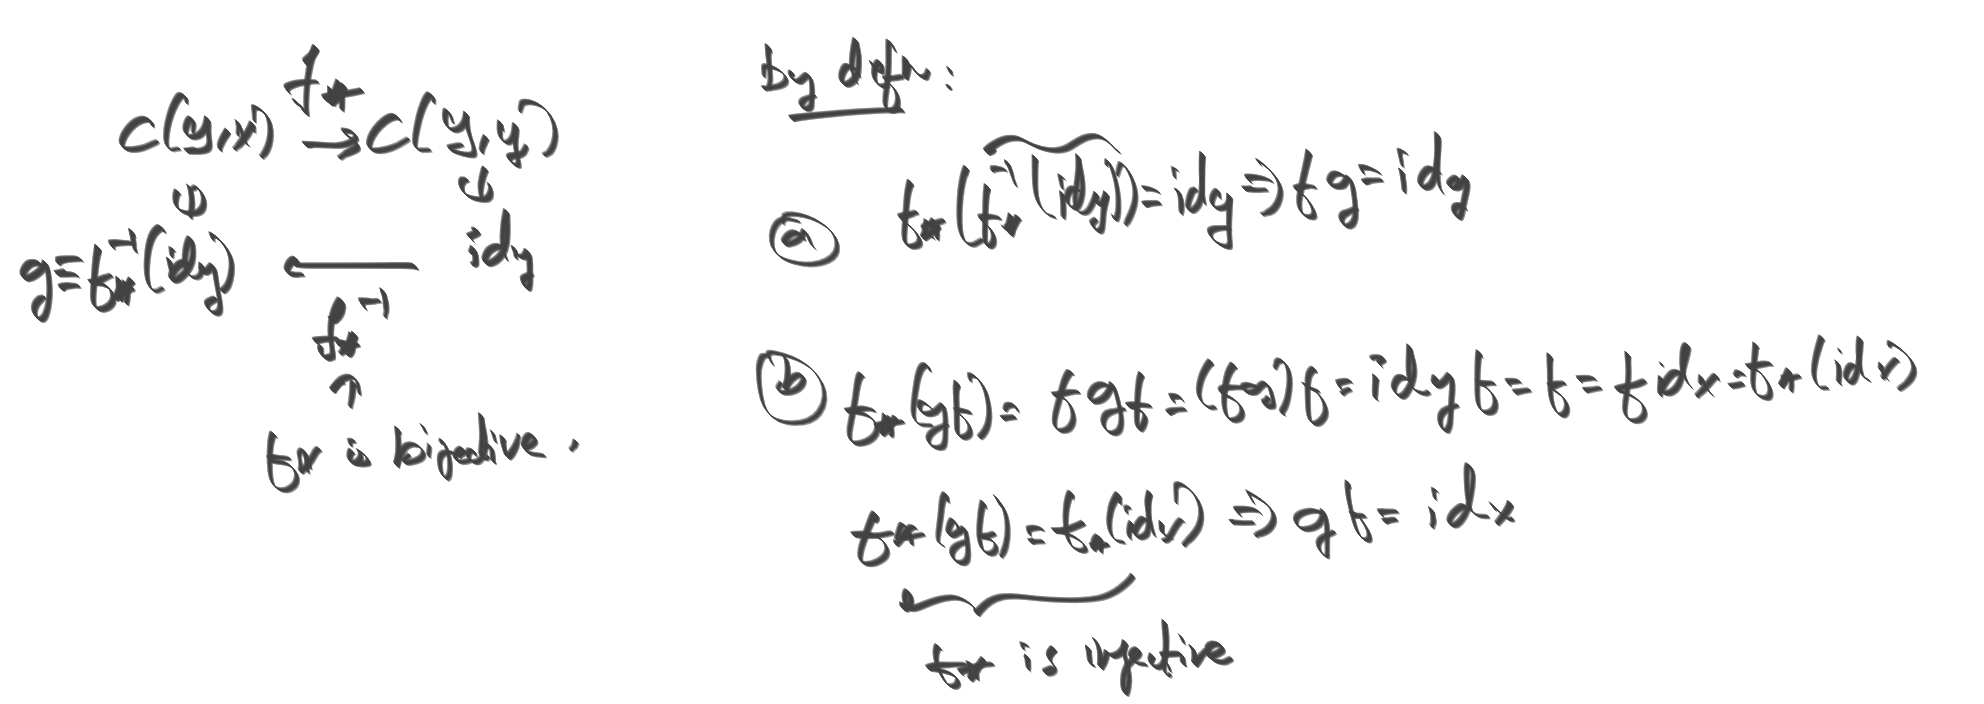
\includegraphics[width=\textwidth]{ch1/iso-is-bijection-of-hom.png}
    \begin{center}Iso is bijection of hom-sets\end{center}
\end{minipage}

\question{Q 1.2.ii:} Show that $f: x \rightarrow y$ is split epi iff for all $c \in C$, post composition
$f \circ - : C(c, x) \rightarrow C(c, y)$ is a surjection.


\proof[(split epi implies post composition is surjective)]
Let $f: e \rightarrow b$ be split epi, and thus possess a section $s: b \rightarrow e$ such that $fs = id_b$.
We wish to show that post composition $C(c, e) \xrightarrow{f_*} C(c, b)$ is surjective.
So pick any $g \in C(c, b)$. Define $sg \in C(c, e)$. See: $$f_*(sg) = fsg = (fs)g = id_b g = g$$.
Hence, for all $g \in C(c, b)$ there exists a pre-image under $f_*$, $sg \in C(c, e)$. Thus, $f_*$ is surjective
since every element of codomain has a pre-image. \qed


\proof[(post composition is surjective implies split epi)]
Let $f: e \to b$ be a morphism such that for all $c \in C$, we have $C(c, e) \xrightarrow{f_*} C(c, b)$ is surjective.
We need to show that there exists a morpshism $s: b \rightarrow e$ such that $fs = id_b$. Set $c = b$.
This gives us a surjection $C(b, e) \xrightarrow{f_*} C(b, b)$. Pick an inverse image of $id_b \in C(b, b)$. 
That is, pick any function $s \in f_*^{-1}(id_b)$. By definition, of $s$ being in the fiber of $id_b$,
we have that $f_*(s) = fs = id_b$. Thus means that we have found a function $s$ such that $fs = id_b$. Thus we are done.
\qed

\question{Q 1.2.iii:} Mono is closed under composition, and if $gf$ is monic then so is $f$.


\proof[(Mono is closed under composition)]
Let $f: x \to y, g: y \to z$ be monomorphisms (Recall that $f$ is a monomorphism iff for any $\alpha, \beta$, if $f \alpha = f \beta$ then $\alpha = \beta$).
We are to show that $gf: x \to z$ is monic.
Consider this diagram which shows that $gfk = gfl$ for arbitrary $k, l: a \to x$. We wish to show that $k=l$.

\begin{minted}{text}
    a --k-> x --f--> y --g--> z
    a --l-> x --f--> y --g--> z
\end{minted}

Since $g$ is mono, we can cancel it from $gfk = gfl$, giving us $fk = fl$.
Since $f$ is mono, we can once again cancel it, giving us $k = l$ as desired.
Hence, we are done.  \qed.

\proof[(If $gf$ is monic then so is $f$)]
Let us assume that $fk = fl$ for arbitrary $l$. We wish to show that $k = l$. We show this
by applying $g$, giving us $fk = fl \implies gfk = gfl$. As $gf$ is monic, we can cancel, giving
us $gfk = gfl \implies k = l$. 
\qed.

\question{Q 1.2.iv} What are monomorphisms in category of fields?

\proof{} Claim: All morphisms are monomorphisms in the category of fields. Let $f: K \rightarrow L$ be an arbitrary field
morphism. Consider the kernel of $f$. It can either be $\{ 0 \}$ or $K$, since those are the only two
ideals of $K$. However, the kernel can't be $K$, since that would send $1$ to $0$ which is an illegal ring map.
Thus, the map $f$ has trivial kernel, therefore is an injection, is left-cancellable, is a monomorphism.\qed


\question{Q 1.2.v} Show that the ring map $i: \mathbb Z \rightarrow \mathbb Q$ is both monic and epic but not iso.

\proof[$i$ is not iso]
No ring map $i: \mathbb Z \rightarrow \mathbb Q$ can be iso since the rings are different (eg. $\mathbb Q$ is a field). \qed



\proof[$i$ is epic]
To show that it's epic, we must show that given for arbitrary $f, g: \mathbb Q \rightarrow R$ that $fi = gi$:

\begin{minted}{text}
Z -i-> Q --f--> R
Z -i-> Q --g--> R
\end{minted}

implies that $f = g$. Let $fi: \mathbb Z \rightarrow R = gi$. Then, the functions $f, g$ are uniquely determined
since $\mathbb Q$ is the field of fractions of $\mathbb Z$, thus a ring map $\Z \rightarrow R$ extends uniquely to a ring
map $\Q \rightarrow R$. Let's assume that $f(i(z)) = g(i(z))$ for all $z$, and show that $f = g$.
Consider arbitrary $p/q \in \mathbb \Q$ for $p, q \in \Z$. Let's evaluate:
\begin{align*}
f(p/q) = f(p)f(q)^{-1} = f(i(p)) \cdot f(i(q))^{-1} = g(i(p)) \cdot g(i(q))^{-1} = g(p/q)
\end{align*}
which shows that $f(p/q) = g(p/q)$ for all $p, q$. Thus, we can extend a ring function defined on the integers to rationals uniquely,
hence $fi = gi \implies f = g$ showing that $i$ is epic.
\qed

\proof[$i$ is monic]
given two arbitrary maps $k, l: R \rightarrow \Z$, if $ik = il$ then we must have $k = l$. Given $ik = il$, since $i$
is an injection of $\Z$ into $\Q$, we must have $k = $l.

\question{Q 1.2.vi} Mono + split epi iff iso.


\proof[Iso is mono + split epi]
Iso is both left and right cancellable. Hence it's mono and epi. It splits because the inverse of the iso splits it. \qed.


\proof[mono + split epi is iso]
Let $f: e \rightarrow b$ be mono (for all $k, l: p \to e$, $fk = fl \implies k = l$)
and split epi (there exists $s: b \rightarrow e$ such that $fs: b \rightarrow b = id_b$.
We need to show it's iso. That is, there exists a $g: b \rightarrow e$ such that $fg = id_b$ and $gf = id_e$.
I claim that $g \equiv s$. We already know that $fg = fs = id_b$ from $f$ being split epi. We need to 
check that $gf = sf = id_a$. Consider:

$$fsf = (fs)f = id_b f = f = f id_e$$

Hence, we have that $f(sf) = f(id_e)$. Since $f$ is mono, we concluce that $sf = id_e$. We are done 
since we have found a map $s$ such that $fs = id_b, sf = id_e$.


\question{1.2.vii} Regarding a poset a category, define the supremum of a subcollection, such that the dual gives the infimum.
\proof{}  We regard an arrow $a \to b$ as witnessing that $a \leq b$. First define an upper bound of a set $O$
to be an object $u$ such that for all $o \in O$, we have $o \leq u$. Now, the supremum of $O$ is the least upper bound
of $O$. That is, $s$ is a supremum iff $s$ is an upper bound, and for all other upper bounds $t$ of $O$, we have that $s \leq t$.
So we draw a diagram showing upper bounds and suprema:

\begin{minipage}{\textwidth}
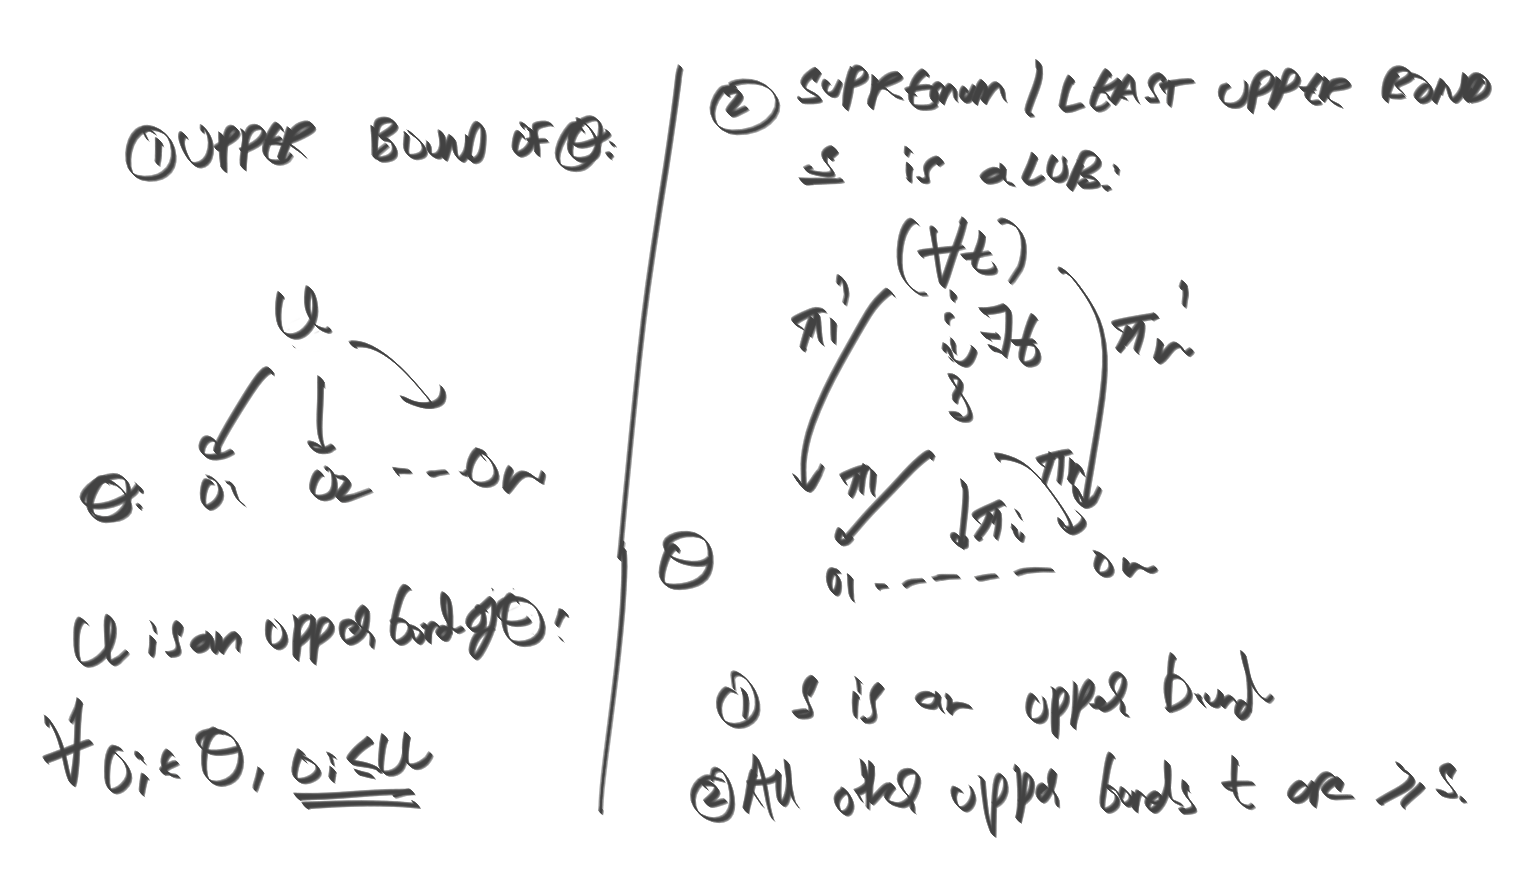
\includegraphics[width=\textwidth]{ch1/sup.png}
    \begin{center}Upper bound and supremum\end{center}
\end{minipage}

\section{Functors}

\question{Exercise 1.3.i}  What is a functor between groups, when regarded as one-object categories?


\proof{} It's going to be a group homomorphism. Since, a functor preserves composition, we have that a
functor $F: C \rightarrow D$ preserves the group structure; for elements of the group / isos $f, g \in Hom(G, G)$, 
we have that the functor obeys $F(f \circ_G g) = (F f) \circ_H (F g)$, which is exactly the equation
we need to preserve group structure. For example, since a functor preserves isomorphisms, an element of the group $f \in Hom(G, G)$
is mapped to an inverbile element $F(f) \in Hom(H, H)$. \qed


\question{Exercise 1.3.ii}  What is a functor between preorders, regarded as a category?

\proof{}Going to be a preorder morphism. I don't know what these are called; If we had a partial order, these
would be called monotone maps. Recall that $a \rightarrow b$ is the encoding of $a \leq b$  within the category.
Suppose we have a functors between preorders (encoded as categories) $F: C \rightarrow D$. Since $F$ preserves
identity arrows, and $a \leq a$ is encoded as $id_a$, we have that $F(a) \leq F(a)$ as:

$$F(a \leq a) = F(id_a) = id_{F(a)} = F(a) \leq F(a)$$


Similarly, since functors take arrows to arrows, the fact that $a \leq b$ which is witnessed by an arrow $a \xrightarrow{f} b$
translates to an arrow $F(a) \xrightarrow{F f} F(b)$, which stands for the relation $F(a) \leq F(b)$. Thus, the map indeed
preserves the preorder structure. Preservation of composition of arrows preserves transitivity of the order relation. \qed


\question{Exercise 1.3.iii} Objects and morphisms in the image of a functor $F: C \rightarrow D$ do not necessarily define a subcategory of $D$.

\proof{} Recall that a morphism can \emph{smoosh} objects, thereby creating coalescing the domains and codomains
of arrows that used to be disjoint. Concretely, consider the diagram:

% https://q.uiver.app/?q=WzAsMTAsWzAsMCwiYSJdLFsxLDAsImIiXSxbMCwxLCJjIl0sWzEsMSwiZCJdLFszLDAsIngiXSxbMywxLCJ6Il0sWzQsMCwieSJdLFszLDIsIng6YSJdLFs0LDIsInk6YixjIl0sWzMsMywiejpkIl0sWzAsMSwiZiJdLFsyLDMsImciXSxbNCw1LCJnIFxcY2lyYyBmIiwyXSxbNiw1LCJsIl0sWzcsOCwiazpmIl0sWzcsOSwiZyBcXGNpcmMgZiIsMl0sWzgsOSwibDpnIl0sWzQsNiwiayJdXQ==
% https://q.uiver.app/?q=WzAsNCxbMCwwLCJhIl0sWzEsMCwiYiJdLFswLDEsImMiXSxbMSwxLCJkIl0sWzIsMywiZyJdLFswLDEsImYiXV0=
\[\begin{tikzcd}
	a & b \\
	c & d
	\arrow["g", from=2-1, to=2-2]
	\arrow["f", from=1-1, to=1-2]
\end{tikzcd}\]

Where we have a category of four objects $a, b, c, d$ with two disconnected arrow $f: a \to b$, and $g: c \to d$.
This is the domain of the functor we will build. The codomain is a three object category:

% https://q.uiver.app/?q=WzAsMyxbMCwwLCJ4Il0sWzEsMCwieSJdLFswLDEsInoiXSxbMCwxLCJrIl0sWzEsMiwibCJdLFswLDIsImxcXGNpcmMgayIsMl1d
\[\begin{tikzcd}
	x & y \\
	z
	\arrow["k", from=1-1, to=1-2]
	\arrow["l", from=1-2, to=2-1]
	\arrow["{l\circ k}"', from=1-1, to=2-1]
\end{tikzcd}\]


The functor will smoosh the four objects into three with a functor, which sends $a$ to $x$, both $b, c$ to $y$, and $d$ to $z$.
Now the image of the functor only has the arrows $k, l$, but not the composite $l \circ k$, which makes the image NOT a subcategory.

% https://q.uiver.app/?q=WzAsMyxbMCwwLCJ4OmEiXSxbMSwwLCJ5OmIsYyJdLFswLDEsIno6ZCJdLFswLDEsIms6ZiJdLFsxLDIsImw6ZyJdLFswLDIsImxcXGNpcmMgazogXFxfIiwyXV0=
\[\begin{tikzcd}
	{x:a} & {y:b,c} \\
	{z:d}
	\arrow["{k:f}", from=1-1, to=1-2]
	\arrow["{l:g}", from=1-2, to=2-1]
	\arrow["{l\circ k: \_}"', from=1-1, to=2-1]
\end{tikzcd}\]



\question{Exercise 1.3.iv} Very that the Hom-set construction is functorial.


\question{Exercise 1.3.v} What is the difference between a functor $F: C^{op} \rightarrow D$ and a functor $F: C \rightarrow D^{op}$?

\proof{} There is no difference. The functor $C^{op} \rightarrow D$ looks like:
% https://q.uiver.app/?q=WzAsNixbMSwwLCJiIl0sWzEsMSwiYSJdLFsyLDAsIkZhIl0sWzIsMSwiRmIiXSxbMCwwLCJhIl0sWzAsMSwiYiJdLFswLDJdLFsxLDNdLFswLDEsImZfe29wfSIsMCx7InN0eWxlIjp7ImJvZHkiOnsibmFtZSI6InNxdWlnZ2x5In19fV0sWzIsMywiRmZfe29wfSJdLFs0LDUsImYiLDJdXQ==
\[\begin{tikzcd}
	a & b & Fa \\
	b & a & Fb
	\arrow[from=1-2, to=1-3]
	\arrow[from=2-2, to=2-3]
	\arrow["{f_{op}}", squiggly, from=1-2, to=2-2]
	\arrow["{Ff_{op}}", from=1-3, to=2-3]
	\arrow["f"', from=1-1, to=2-1]
\end{tikzcd}\]

while the functor $G: D \rightarrow C^{op}$ looks like:

% https://q.uiver.app/?q=WzAsNixbMCwwLCJwIl0sWzAsMSwicSJdLFsxLDAsIkdwIl0sWzEsMSwiR3EiXSxbMiwwLCJHcCJdLFsyLDEsIkdxIl0sWzAsMSwiZiJdLFswLDJdLFsyLDMsIkdmIiwyLHsic3R5bGUiOnsiYm9keSI6eyJuYW1lIjoic3F1aWdnbHkifX19XSxbMSwzXSxbNSw0LCJHZiIsMl1d
\[\begin{tikzcd}
	p & Gp & Gp \\
	q & Gq & Gq
	\arrow["f", from=1-1, to=2-1]
	\arrow[from=1-1, to=1-2]
	\arrow["Gf"', squiggly, from=1-2, to=2-2]
	\arrow[from=2-1, to=2-2]
	\arrow["Gf"', from=2-3, to=1-3]
\end{tikzcd}\]

Given a functor $F: C^{op} \rightarrow D$, we can build an associated functor $G_F: C \rightarrow D^{op}$. Consider
an arrow $x \rightarrow{f} y \in C$ . Dualize it, giving us an arrow $y_{op} \xrightarrow{f_{op}} x_{op} \in C^{op}$. Find
it image under $F$, which gives us an arrow $F(y_{op}) \xrightarrow{F(f_{op})} F(x_{op}) \in D$. Dualize this
in $D$, giving us $F(x_{op})_{op} \xrightarrow{F(f_{op})}_{op} F(y_{op}) \in D^{op}$. See that the arrow
direction coincides with the domain arrow direction $x \rightarrow{f} y \in C$. So we can build a functor $H$
which sends the arrow $x \rightarrow{f} y \in C$ to the arrow $F(x_{op})_{op} \xrightarrow{F(f_{op})}_{op} F(y_{op}) \in D^{op}$.
Hence, $H: C \rightarrow D^{op}$, defined by $H(x) \equiv F(x_{op})_{op}$ and $H(f) \equiv F(f_{op})_{op}$. 
By duality, we get the other direction where we start from $F': C \rightarrow D^{op}$ and end at $H': C^{op} \rightarrow D$.
Thus, the two are equivalent.

In a nutshell, the diagram is:

% https://q.uiver.app/?q=WzAsMTUsWzEsMCwiYiJdLFsxLDEsImEiXSxbMiwwLCJGYiJdLFsyLDEsIkZhIl0sWzAsMCwiYSJdLFswLDEsImIiXSxbNCwwLCJhIl0sWzQsMSwiYiJdLFs1LDAsIkZhIl0sWzUsMSwiRmIiXSxbNywwLCJGYiJdLFs3LDEsIkZhIl0sWzMsMCwiXFxpbXBsaWVzIl0sWzMsMSwiXFxpbXBsaWVzIl0sWzYsMF0sWzAsMl0sWzEsM10sWzAsMSwiZl97b3B9IiwwLHsic3R5bGUiOnsiYm9keSI6eyJuYW1lIjoic3F1aWdnbHkifX19XSxbMiwzLCJGZl97b3B9Il0sWzQsNSwiZiIsMl0sWzYsNywiZiJdLFs2LDhdLFs4LDksIihGZilfe29wfSIsMCx7InN0eWxlIjp7ImJvZHkiOnsibmFtZSI6InNxdWlnZ2x5In19fV0sWzcsOV0sWzEwLDExLCJGZl97b3B9Il1d
\[\begin{tikzcd}
	a & b & Fb & \implies & a & Fa & {} & Fb \\
	b & a & Fa & \implies & b & Fb && Fa
	\arrow[from=1-2, to=1-3]
	\arrow[from=2-2, to=2-3]
	\arrow["{f_{op}}", squiggly, from=1-2, to=2-2]
	\arrow["{Ff_{op}}", from=1-3, to=2-3]
	\arrow["f"', from=1-1, to=2-1]
	\arrow["f", from=1-5, to=2-5]
	\arrow[from=1-5, to=1-6]
	\arrow["{(Ff)_{op}}", squiggly, from=1-6, to=2-6]
	\arrow[from=2-5, to=2-6]
	\arrow["{Ff_{op}}", from=1-8, to=2-8]
\end{tikzcd}\]



\question{Exercise 1.3.vi} Given the comma category $F \downarrow G$, define the domain and codomain projection functors $dom: F \comma G \rightarrow F$
  and $codom: F \comma G \rightarrow G$.


Recall that an object in the comma category is a a triple $(d \in D, e \in E, F(d) \xrightarrow{f} F(e))$, or diagramatically:

% https://q.uiver.app/?q=WzAsNCxbMCwwLCJkIFxcaW4gRCJdLFsxLDAsImUgXFxpbiBFIl0sWzAsMSwiRmRcXGluIEMiXSxbMSwxLCJHZSBcXGluIEMiXSxbMCwyLCJGOiBEICIsMl0sWzEsMywiRyJdLFsyLDMsImYiLDJdXQ==
\[\begin{tikzcd}
	{d \in D} & {e \in E} \\
	{Fd\in C} & {Ge \in C}
	\arrow["{F: D }"', from=1-1, to=2-1]
	\arrow["G", from=1-2, to=2-2]
	\arrow["f"', from=2-1, to=2-2]
\end{tikzcd}\]

and a morphism in such a category is a diagram:

% https://q.uiver.app/?q=WzAsNyxbMSwwLCJGZCJdLFsyLDAsIkdlIl0sWzEsMiwiRmQnIl0sWzIsMiwiR2UnIl0sWzAsMiwiKGQnLCBlJyxmJykiXSxbNSwyXSxbMCwwLCIoZCwgZSxmKSJdLFsyLDMsImYnIiwyXSxbMCwxLCJmIiwyXSxbMCwyLCJcXGFscGhhIiwxXSxbMSwzLCJcXGJldGEgIiwxXSxbNiw0LCIoXFxhbHBoYSBcXGRvd25hcnJvdyBcXGJldGEpIiwxXV0=
\[\begin{tikzcd}
	{(d, e,f)} & Fd & Ge \\
	\\
	{(d', e',f')} & {Fd'} & {Ge'} &&& {}
	\arrow["{f'}"', from=3-2, to=3-3]
	\arrow["f"', from=1-2, to=1-3]
	\arrow["\alpha"{description}, from=1-2, to=3-2]
	\arrow["{\beta }"{description}, from=1-3, to=3-3]
	\arrow["{(\alpha \downarrow \beta)}"{description}, from=1-1, to=3-1]
\end{tikzcd}\]

We constrct the domain functor $dom$ as a functor that sends an object $(d \in D, e \in E, F(d) \xrightarrow{f} F(e))$ to an object $d \in D$.
It sends the morphism between $(d, e, f)$ and $(d', e', f')$, given by $(\alpha : Fd \rightarrow Fd', \beta: Ge \rightarrow Ge')$ to
the arrow $Fd \xrightarrow{\alpha} Fd' \in D$.

In a diagram, this looks like:

% https://q.uiver.app/?q=WzAsMTAsWzEsMCwiRmQiXSxbMiwwLCJHZSJdLFsxLDIsIkZkJyJdLFsyLDIsIkdlJyJdLFswLDAsIihkLCBlLGYpIl0sWzAsMiwiKGQnLCBlJyxmJykiXSxbNSwyXSxbMywxLCJcXHhyaWdodGFycm93e2RvbX0iXSxbNCwwLCJGZCJdLFs0LDIsIkZkJyJdLFsyLDMsImYnIiwyXSxbMCwxLCJmIiwyXSxbMCwyLCJcXGFscGhhIiwxXSxbMSwzLCJcXGJldGEgIiwxXSxbNCw1LCIoXFxhbHBoYSBcXGRvd25hcnJvdyBcXGJldGEpIiwxXSxbOCw5LCJcXGFscGhhIiwxXV0=
\[\begin{tikzcd}
	{(d, e,f)} & Fd & Ge && Fd \\
	&&& {\xrightarrow{dom}} \\
	{(d', e',f')} & {Fd'} & {Ge'} && {Fd'} & {}
	\arrow["{f'}"', from=3-2, to=3-3]
	\arrow["f"', from=1-2, to=1-3]
	\arrow["\alpha"{description}, from=1-2, to=3-2]
	\arrow["{\beta }"{description}, from=1-3, to=3-3]
	\arrow["{(\alpha \downarrow \beta)}"{description}, from=1-1, to=3-1]
	\arrow["\alpha"{description}, from=1-5, to=3-5]
\end{tikzcd}\]

$codom$ will do the same thing, by stripping out the codomain of the comma instead of the domain. \qed

\question{Exercise 1.3.vii} Define slice category as special case of the comma category.


\proof{} To define the slice $C/c$ whose objects are of the form $d \rightarrow c$ for varying $d \in C$, we pick
the category $D = C, E = C$, and functors $F : C \rightarrow C = id$, $G : C \rightarrow C = \delta_c$, that is, the constant functor
which smooshes the entire $C$ category into the object $c \in C$ by mapping all objects to $c$ and all arrows to $id_{c}$.

This causes the diagram to collapse down to objects of the form $d \rightarrow c$, and the arrows to be what we'd expect \qed.

\question{Exercise 1.3.viii} Show that functors need not reflect isomorphisms. for a functor $F: C \rightarrow D$, and a 
morphisms $f \in C$ such that $F f$ is an isomorphism in $D$ but $f$ is not an isomorphism in $C$.


Pick a category $C$ and an object $o \in C$. Build the constant functor $\delta_o: C \rightarrow C$. The image
of every arrow $c \xrightarrow{a} c'$ is the identity arrow $id_o$ which is an iso. The arrow $a$ need not be iso. The functor
$\delta_o$ does not reflect isos. \qed

\question{Exercise 1.3.ix} Consider the not-yet-functors $Grp \rightarrow Grp$ that sends a group to its center, comutator subgroup, and automorphism group.
Are these functors if we limit the category $Grp$ to have (a) only isomorphisms? (b) only epimorphisms? (c) all homomorphisms?

\proof[(isos)] If we have (a) only isomorphisms, then these are indeed functors, since an isomorphism $G \simeq H$
implies that their group theoretic properties are identical. Thus, we will have
$Z(G) \simeq Z(H)$, ie, isomorphic centers.
Thus, an iso arrow $f: G \rightarrow H$ becomes an iso arrow
$Z(f) : Z(G) \rightarrow Z(H)$. The exact same happens for commutator and automorphism. \qed

\proof[(epis)] If we only have epimorphisms, we first invoke  given footnote 29, that all
epis in Group are surjections. Thus, given an epi (surjection) $\phi: G \twoheadrightarrow H$, we
identify $im(\phi) \simeq G/ker(\phi)$ or $H \simeq G/ker(\phi)$, since $H \simeq im(\phi)$ by $\phi$ being a surjection.
So we can choose to study only quotient maps $\phi: G \rightarrow G/ker \phi$.

For the center, consider the determinant map $|\cdot|: GL(2, \mathbb R) \rightarrow \mathbb R^\times$.
This map is surjective since we can pick the matrix $\begin{bmatrix} 1 & 0 \\ 0 & r \end{bmatrix}$ to get all possible
determinants  for arbitrary $r \in \mathbb R$. The center
of the group of matrices is scalar multiples of the identity, thus $Z(GL(2, \mathbb R)) = \{ k I : k \in \mathbb R \}$.
The center of the reals $Z(\mathbb R^\times)$ is the reals themselves since it's an abelian group. Now see
that the determinant of a matrix $kI$ must be $k^2$, since we get two copies of $k$ along the diagonal. Thus, the image
$\phi(Z(GL(2, \mathbb R))) = \{ k^2 : k \in \mathbb R \} = \mathbb R_{\geq 0}$ which is smaller than the center of the image,
$Z(\phi(GL(2, \mathbb R))) = Z(\mathbb R^{\times}) = \mathbb R^\times$. Thus, \textbf{the center not functorial on epis}.

\section{Natural Transformations}

\subsection{Musing}
\subsubsection{Torsion decomposition}

Let $TA$ be the subgroup of $A$ that have finite order.

\begin{itemize}
\item The idea is to first show that any natural transformation of the identity functor $\eta: 1 \implies 1$ is multiplication by some $n \in \Z$
(recall that every abelian group is a \Z-module, so this is a sensible thing to say).
\item Let's study the component of $\eta$ at $\mathbb Z$.
This means that we have an arrow at $1(\Z) \xrightarrow{\eta(id)} 1(\Z)$, which is $\Z \rightarrow{\eta(id)} \Z$ since identity functor
leaves objects and arrow invariant. Any arrow $\Z \xrightarrow{\eta(id)} \Z$ is a multiplication by some natural number.
\item Now consider a homomorphism $f: \Z \rightarrow A$. This is determined entirely by $f(1) \in A$, so any such map is 
  the same as picking an element $a \in A$. 
\item Let's now consider the isomorphism $A \epi A/TA \mono TA \oplus (A/TA) \simeq A$. If this isomorphism were natural,
    then we would have a natural endomorphism of the identity functor $\alpha: 1 \rightarrow 1$.
\item Let's observe $\alpha$ at $\mathbb Z$. We already know that such a transformation is given by $\Z \xrightarrow{\alpha} \Z$,
    which is multiplication b a number $n \neq 0$ (can't be zero since we need an isomorphism).
\item Now consider $C \equiv \Z/2n\Z$ where $n$ is the $\alpha$ scale factor. See that $T(\Z/2n\Z) = \Z/2n\Z$.
    So we get the factoring as $\Z/2n\Z \epi 0 \mono \Z/2n\Z \oplus 0 \simeq \Z/2n\Z$. Since we factor through zero,
    the full map is the zero map. However, we know from the natural transformation that the natural transformation 
    must scale all elements by $n \neq 0$. So we break naturality
\end{itemize}

The big thing I don't understand in this is why we need to factor \emph{through} the epi. If I directly define
$A \rightarrow (A/TA) \oplus TA$, given by the exact sequence $0 \mono TA \mono A \epi A/TA \epi 0$? Ah I see, this sequence
need not always split. 


\subsection{Exercises}

\question{Exercise 1.4.i} Let $\alpha: F \nt G$ be a natural isomorphism. Show that the inverses of the components define a natural isomorphism $\inv\alpha: G \nt F$.

\question{Exercise 1.4.ii} What is a natural transformation between a parallel pair of functors between groups regarded as one object categories?

\proof{} Let $G, H$ be groups regarded as one object categories, so elements are arrows. A functor $F: G \rightarrow H$ is a group homomorphism. Two functors $F, F': G \rightarrow H$
are two group homomorphisms. An natural transformation is a map $\eta: G \rightarrow H$ which for every (the only) object $*_G \in G$, assigns
an arrow $\eta(*_G): F(*_G) \xrightarrow{\eta(*_G)} G(*_G)$ which is compatible with all arrows:

% https://q.uiver.app/?q=WzAsNSxbMCwwLCJGKCopIFxcaW4gSCJdLFsxLDAsIkYnKCopIFxcaW4gSCJdLFswLDEsIkYoKikgXFxpbiBIIl0sWzEsMSwiRicoKikgXFxpbiBIIl0sWzEsMl0sWzAsMSwiXFxldGEoKikiXSxbMiwzLCJcXGV0YSgqKSJdLFswLDIsIkYoaCkiLDFdLFsxLDMsIkYnKGgpIiwxXV0=
\[\begin{tikzcd}
	{F(*_G) \in H} & {F'(*_G) \in H} \\
	{F(*_G) \in H} & {F'(*_G) \in H} \\
	& {}
	\arrow["{\eta(*_G)}", from=1-1, to=1-2]
	\arrow["{\eta(*_G)}", from=2-1, to=2-2]
	\arrow["{F(g)}"{description}, from=1-1, to=2-1]
	\arrow["{F'(g)}"{description}, from=1-2, to=2-2]
\end{tikzcd}\]

Simplifying the diagram by substituting $F(*) = F'(*) = *$, and setting $\alpha \equiv \eta(*G) \in Hom(*_H, *_H)$, we get:

% https://q.uiver.app/?q=WzAsNSxbMCwwLCIqX0giXSxbMSwwLCIqX0giXSxbMCwxLCIqX0giXSxbMSwxLCIqX0giXSxbMSwyXSxbMCwxLCJcXGFscGhhIFxcZXF1aXYgXFxldGEoKl9HKSJdLFsyLDMsIlxcYWxwaGEgXFxlcXVpdiBcXGV0YSgqX0cpIiwyXSxbMSwzLCJGJyhoKSJdLFswLDIsIkYoaCkiLDJdXQ==
\[\begin{tikzcd}
	{*_H} & {*_H} \\
	{*_H} & {*_H} \\
	& {}
	\arrow["{\alpha \equiv \eta(*_G)}", from=1-1, to=1-2]
	\arrow["{\alpha \equiv \eta(*_G)}"', from=2-1, to=2-2]
	\arrow["{F'(g)}", from=1-2, to=2-2]
	\arrow["{F(g)}"', from=1-1, to=2-1]
\end{tikzcd}\]

So we are looking for an arrow (group element) $\alpha \in H$ such that for all $g \in G$, $F'(g) \cdot \alpha = \alpha \cdot F(g)$.
On rearranging: $\alpha^{-1} \cdot F'(g) \cdot \alpha = F(g)$. So it gives a sort of  ``inner automorphism'' from $F$ to $F'$. \qed


\question{Exercise 1.4.iii} What is a natural transformation between a parallel pair of functors between preorders regarded as categories?
\proof We regard preorders as thin categories, where there is an most arrow from $p \rightarrow p'$ if $p \leq p'$. A functor from $(P, \leq)$ to $(Q, \leq)$
is a monotone map. A pair of functors $F, G: P \rightarrow Q $ is a pair of monotone maps. A natural transformation $\eta: F \nt G$ makes for each $p \in $P
the diagram commute:

% https://q.uiver.app/?q=WzAsNixbMiwwLCJGKHApIl0sWzMsMCwiRyhwKSJdLFsyLDEsIkYocSkiXSxbMywxLCJHKHEpIl0sWzAsMCwicCJdLFswLDEsInEiXSxbMCwxLCJcXGV0YShwKSJdLFsyLDMsIlxcZXRhKHEpIl0sWzAsMiwiRihwPHEpIiwyXSxbMSwzLCJHKHAgPCBxKSJdLFs0LDUsInA8IHEiXV0=
\[\begin{tikzcd}
	p && {F(p)} & {G(p)} \\
	p' && {F(p')} & {G(p')}
	\arrow["{\eta(p)}", from=1-3, to=1-4]
	\arrow["{\eta(p)}", from=2-3, to=2-4]
	\arrow["{F(p<p')}"', from=1-3, to=2-3]
	\arrow["{G(p < p')}", from=1-4, to=2-4]
	\arrow["{p< p'}", from=1-1, to=2-1]
\end{tikzcd}\]

So, for every $p \leq p'$, the functor $F$ maps us to elements $F(p) \leq F(p')$, and $G$ maps us to elements $G(p) \leq G(p')$. The natural transformation $\eta$
asks to witness an arrow $F(p) \xrightarrow{\eta(p)} G(p)$, which means that we must have $F(p) \leq G(p)$ within the category $Q$, and similarly for $p'$.
Thus, it witnesses that $G$ is always \emph{above} $F$. For any element $p \in P$, we will always have $F(p) \leq G(p)$, in a way that is consistent with the
monotonicity of $F, G$.


\question{Exercise 1.4.iv} Prove that distinct parallel morphisms $f, g: c^\to_\to d$ define distinct natural transformations $f_*, g_*: C(-, c) \nt C(-, d)$ by pre-composition.
\end{document}
